\documentclass[
	letterpaper
	12pt
]{template}
\usepackage{wrapfig}
\usepackage{apacite}
\usepackage{titling}
\usepackage{multicol}
\usepackage{caption}


\usepackage[font=footnotesize,labelfont=bf]{caption}

\setlength{\droptitle}{-10em}

\newcommand{\bref}[2]{\textbf{\hyperref[#1]{#2}}}

\title{Blackbody Radiation}

\author{Sebastien Psarianos, Yuchen Jiang}

\date{\today}



\begin{document}
\maketitle
\section{Abstract}
In this report, we evaluate the effectiveness of the Wien Displacement Law and the Stefan-Boltzmann equation through emission spectrum analysis of a black body at varying temperatures. Using a prism photospectrometer setup, we performed spectral decomposition of blackbody light emissions. We inferred the temperature of the black body by measuring the power supplied to it and used this information to approximate the intensity and the peak wavelength across varying temperatures. By varying the supply voltage to the black body, we were able to compare the emissions spectrums at differing temperatures. Through the course of this analysis we were able to verify the predictions of Wien's Law, achieving a $\chi_{red}^2$ value of 0.676 and a reasonable level of precision on our fit variables. We were unsucessful in verification of the Stefan-Boltzmann equation due to the inaccuracy of our intensity approximation model. A study into intensity approximation would provide a more insightful result for this model.



\section{Introduction}
\subsection{Background}
In this lab, we study two key characteristics of the black body emission spectrum and how they vary with temperature. The first metric is the wavelength where the emission intensity distribution peak occurs ($\lambda_{\rm max}$). Theoretically, this wavelength is related to the temperature of the black body ($T$) through Wien's Displacement law \cite{labManual}:
\begin{equation}\label{eqn::wien}
	\lambda_{\rm max} = {1\over T} \cdot 2.989\times 10^{-3}\unit{m\cdot K}
\end{equation}
The second metric is the total intensity of light that is emitted by the black body over the entire spectrum ($I$). This value is related to the temperature of the black body ($T$) by the Stefan-Boltzmann equation \cite{labManual}:
\begin{equation}\label{eqn::stefan}
	I = \epsilon \cdot \sigma \cdot T^4
\end{equation}
Where $\epsilon$ is known as the emissivity of the surface of the body. $\epsilon=1$ for the idealized black body and $\epsilon < 1$ for most materials. $\sigma = 5.67\times10^{-8}\unit{W \cdot m ^{-2} \cdot K^{-4}}$ is the Stefan-Boltzmann constant \cite{labManual}. For a black body that is heated through an electric current with voltage $V$ and current $I$, the temperature is given by: \cite{labManual}
\begin{equation}\label{eqn::temp}
	T = T_0 + {1\over \alpha_0}\left({{V/I\over R_0}-  1}\right)
\end{equation}
Where $\alpha_0=4.5\times10^{-3}\unit{\per \kelvin}$ and $R_0 = 1.1\Omega$ for our apparatus and $T_0$ is room temperature.
\subsection{Using refraction to perform spectral decomposition}\label{sec::refraction}
\begin{wrapfigure}{r}{0.4\textwidth}\label{fig::refract}
	\vspace{-15pt}
	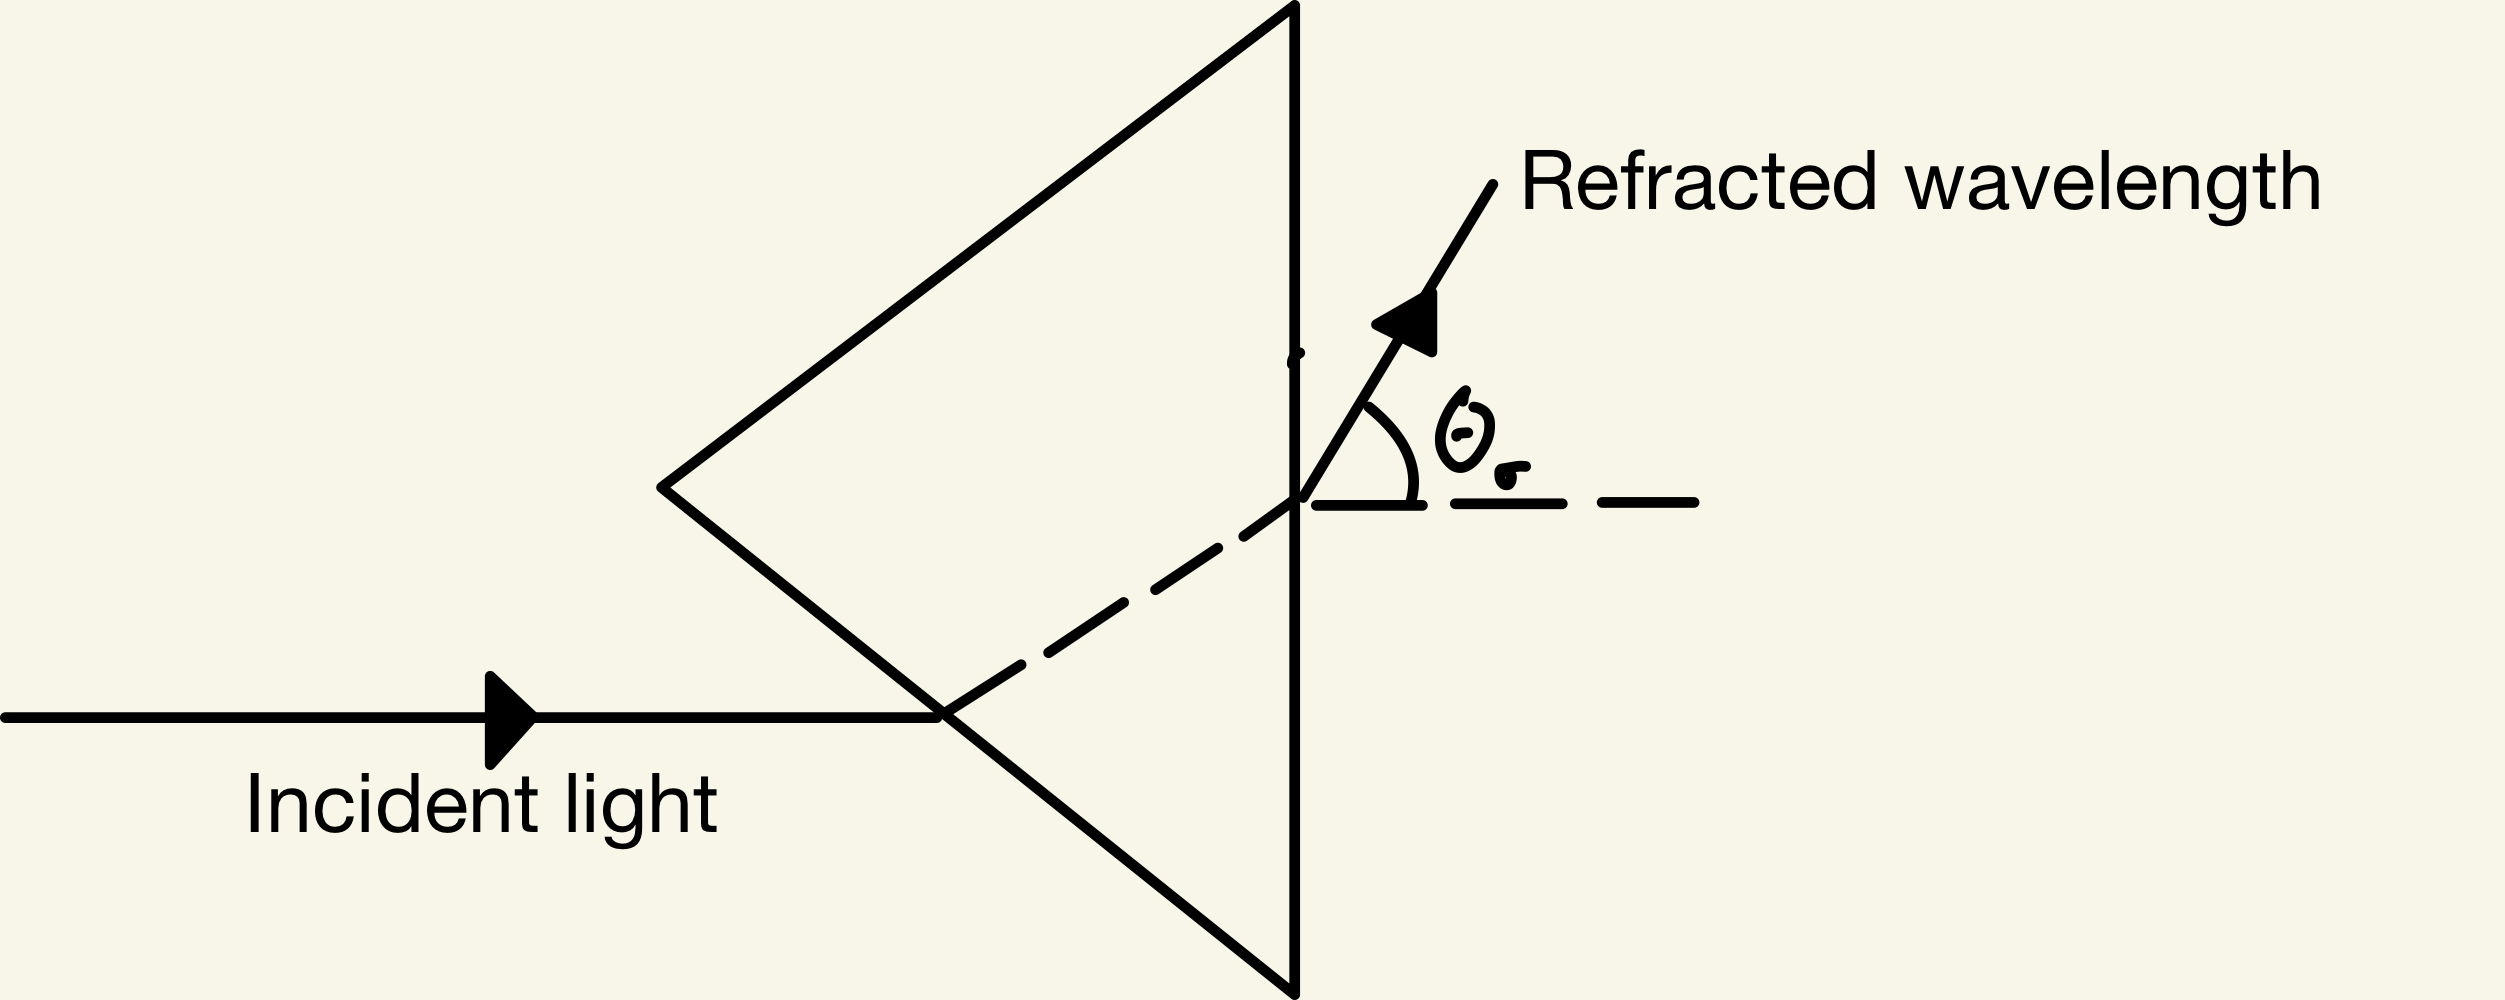
\includegraphics[width=.4\textwidth]{img/refract.png}
	\caption{Diagram of prism refraction}
	\vspace{-20pt}
\end{wrapfigure}
To determine the effectiveness of these models, the emitted light from the black body must first be separated into a spectrum of its constituent wavelengths. By refracting the light through a triangular prism as shown in \bref{fig::refract}{Figure 1}, every wavelength of light that is present will refract with a different refraction angle ($\theta_r$).\vspace{\baselineskip}

Snell's law can be applied to this system, both on the refraction angle $(\theta_r)$ and the $60\unit{^o}$ incident angle. This gives the refraction index $n$ as a function of $\theta_r$. \cite{labManual}
\begin{equation}\label{eqn::index}
n(\theta_r) = \sqrt{\left({2\over \sqrt 3}\sin\theta_r + {1\over 2} \right) + {3\over 4}}
\end{equation}
The Cauchy equation can be rearranged to give the wavelength $\lambda$ corresponding to a refraction index $n$ \cite{labManual}
\begin{equation}\label{eqn::cauchy}
	\lambda = \sqrt{A\over {n-B}}
\end{equation}
For our apparatus $A = 13900$ and $B=1.689$. This creates a spectral decomposition for different angles relative to the prism. \bref{eqn::index}{Equation 4} and \bref{eqn::cauchy}{Equation 5} can be used to convert the angle a sample is detected at to its refraction index and then to its original wavelength.
\subsection{The experiment}
In this report, we aim to quantify the accuracy of the \bref{eqn::wien}{Wien Displacement Law} and the \bref{eqn::stefan}{Stefan-Boltzmann equation}. This is done by comparing their predictions of the blackbody emission spectrum with experimental results. By measuring the intensity of the blackbody light as a function of refraction angle through a triangular prism, we can infer the original wavelengths using \bref{eqn::index}{Snell's Law} and \bref{eqn::cauchy}{The Cauchy Equation}. This will produce a plot of the emission spectrum. We can analyze this to determine the total energy $I$ and the max refraction wavelenth $\lambda_{\rm max}$ to verify theoretical predictions.
\section{Methodology}
\subsection{Apparatus}
\begin{wrapfigure}{r}{0.4\textwidth}\label{fig::apparatus}
	\vspace{-15pt}
	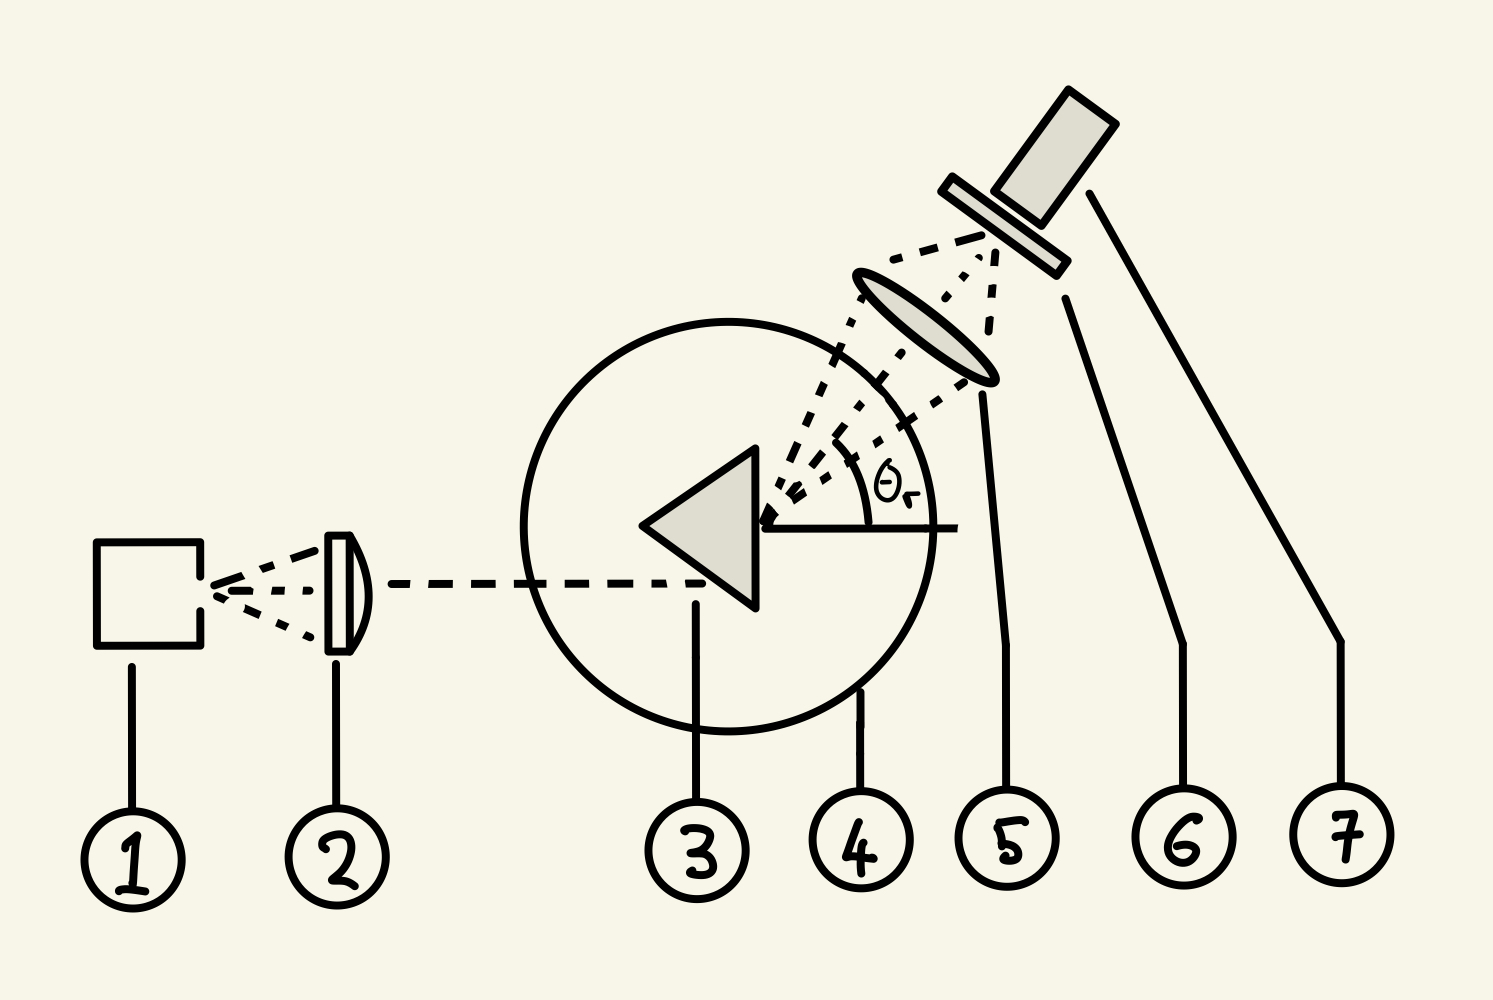
\includegraphics[width=.4\textwidth]{img/apparatus.jpeg}
	\caption{Diagram of PASCO OS-8537 Spectrophotometer: 1-Blackbody source, 2-Collimating Lens, 3-Refraction Prism, 4-Angle indicator, 5-Focusing Lens, 6-Variable Aperture, 7-Light intensity meter}
	\vspace{-20pt}
\end{wrapfigure}
In this study we examine the properties of blackbody radiation using a Prism photospectrometer, namely the PASCO OS-8537. A diagram of this system is shown in  \bref{fig::apparatus}{Figure 2}. This apparatus applies the principles of prism refraction discussed in \bref{sec::refraction}{Section 2.2} to decompose the black body emissions into a spectrum of wavelengths with specific refraction angles $\theta_r$. The focusing lens, variable aperture, and light intensity meter (5, 6, 7 in \bref{fig::apparatus}{Figure 2}) were mounted on an arm that was able to swing around the pendulum to vary $\theta_r$. \vspace{\baselineskip}

Data collection is supported by a LabVIEW program created to capture the spectrum. The software includes functions for data refinement, minimizing background noise interference and ensuring the data accurately represents the signal rather than external factors or electronic disruptions.\vspace{\baselineskip}

This application measures the intensity of light versus the angle of the light detector arm from its position at the start of the sample in a clockwise direction $(\theta)$. In addition, it measured the voltage and current used by the blackbody source. This provided us a plot of light intensity measured by the detector vs angle, and the required information to calculate the blackbody temperature using \bref{eqn::temp}{Equation 3}.
\subsection{Minimizing Interference}
The variable aperture (6 in \bref{fig::apparatus}{Figure 2}) was set to Slit \#3. The collimating lens (2 in \bref{fig::apparatus}{Figure 2}) was placed  10 cm from the blackbody source (1 in \bref{fig::apparatus}{Figure 2}) to guarantee parallel light beams into the prism. This is essential for spectral dispersion \cite{labManual}. The  focusing lens position (5 in \bref{fig::apparatus}{Figure 2}) and the intensity meter amplification were adjusted through trial runs to minimize the noise in the LabVIEW plot. These initial configurations were done to deliver a focused spectrum that accurately represented the blackbody emissions while maintaining a balance between light transmission and resolution.
\subsection{Experimental Procedure}
We took two sets of data to analyse for the purpose of verifying both \bref{eqn::wien}{Equation 1} and \bref{eqn::stefan}{Equation 2}. The LabVIEW application allowed us to choose the voltage supplied to the black body for each trial and select either a $30\unit{^o}$ or $80\unit{^o}$ measurement arc. \vspace{\baselineskip}

For the first data set, we took five samples each at V = \{4.0, 5.0, 6.0, 7.0, 8.0, 9.0, 10.0\}{V} as indicated in the application, each with an $80\unit{^o}$ measurement arc, giving 35 data points. For each of these samples, the arm on the apparatus was set to be at the $0$ degree point almost parallel to the prism's right face. After selecting the appropriate starting values, we slowly rotated the arm until the measurement was finished. We then exported the data to a txt file and noted down the voltage and current displayed in the software into a spreadsheet.\vspace{\baselineskip}

For the second data set, we took five samples each at V = \{4.0, 5.0, 6.0, 7.0, 8.0, 9.0, 10.0\}{V} as indicated in the application, each with a $30\unit{^o}$ measurement arc, giving 35 data points. The same procedure was followed as the previous data set, however the measurement arc was significantly shorter.
\section{Results}
\subsection{First Data set}
\begin{wrapfigure}{r}{0.3\textwidth}\label{fig::peaks}
	\vspace{-27pt}
	\includegraphics[width=.3\textwidth]{../python/output/wein/peaks/26.pdf}
	\caption{Plot of raw data from example 80 degree trial. First vertical line shows $\theta_{max}$ and second vertical line shows $\theta_0$}
	\vspace{-20pt}
\end{wrapfigure}
Every sample that was measured had two peaks, one large peak and one small peak. The large peak was the peak of the emission spectrum, whereas the small peak is produced by a small amount of light that passes over the prism. By using the find\_peaks function from the scipy.signal package, we were able to determine the angles where both of these peaks occurred. This gave $\theta_{max},\theta_{0}$ the angle of the larger and smaller peaks respectively for each sample.\vspace{\baselineskip}

$\theta_r$ can be calculated from these two angles. $\theta_0$ will be perpendicular to the right face of the pendulum, therefore it acts as a zero position for $\theta_0$. Therefore, $\theta_r$ is given: $\theta_r =\theta_{0} - \theta_{max}$. The value $\theta_r$ was then converted to $\lambda_{\rm max}$ as described in \bref{sec::refraction}{Section 2.2}. The voltage and current readings were used in conjunction with \bref{eqn::temp}{Equation 3} to calculate the temperature of the black body.\vspace{\baselineskip}

\begin{wrapfigure}{r}{0.4\textwidth}\label{fig::expOne}
	\vspace{-15pt}
	\includegraphics[width=.4\textwidth]{../python/output/wein/lambdaVsTemps.pdf}
	\caption{Plot of mean peak wavelength versus mean temperature for a blackbody emission spectrum. Plotted values are the mean of five samples at a single voltage with error given by the standard deviation of these samples. An inverse best fit is included to reflect \bref{eqn::wien}{Equation 1} }
	\vspace{-50pt}
\end{wrapfigure}
The mean temperature and mean $\lambda_{\rm max}$ were calculated from the five samples at each voltage value. This was plotted in \bref{fig::expOne}{Figure 4}. Uncertainty was calculated for both temperature and $\lambda_{\rm max}$ by taking the std deviation of the five samples at each voltage level. The fit was done using the following python function to simulate \bref{eqn::wien}{Equation 1}:
\begin{lstlisting}[label={fnc::invFit},captionpos=b,language=python]
	def invFit(x, A):
    return A/x
\end{lstlisting}
The resulting fit coefficient was $(2.35\pm 0.04)\times10^{-3} \unit{m\cdot K}$ with a $\chi_{\rm red }^2 = 0.676$. The order of magnitude of this result is identical to the theoretical value in \bref{eqn::wien}{Equation 1} of $ 2.989\times 10^{-3}\unit{m\cdot K}$, however there is a discrepancy of $\approx 6.4\times10^{-4}$.\vspace\baselineskip

\bref{fig::expOneRes}{Figure 5} shows the residuals plot for \bref{fig::expOne}{Figure 4}. Visually, there is no clear trend in the residuals, which suggests that the deviation from the model could be due to noise in the environment rather than some higher order term that is causing small deviations. \vspace{\baselineskip}

\begin{wrapfigure}{r}{0.4\textwidth}\label{fig::expOneRes}
	\vspace{-20pt}
	\includegraphics[width=.4\textwidth]{../python/output/wein/lambdaVsTempsResidual.pdf}
	\caption{Residuals plot for \bref{fig::expOne}{Figure 4}}
	\vspace{-20pt}
\end{wrapfigure}
Considering the low $\chi_{\rm red}^2$ metric and the lack of trends in the residuals, the data seems to suggest that the inverse relationship suggested in \bref{eqn::wien}{Equation 1} between temperature and wavelength is a good model to describe the peak black body emission spectrum. The small discrepancy between the fit coefficients and the theoretical value still presents an issue with the model. \vspace\baselineskip

The uncertainty in this experiment was relatively high in comparison to the data, especially for the $\lambda_{\rm max}$ measurements. The uncertainty was calculated in terms of standard deviation of a sample of results, and $\lambda_{\rm max}$ was inferred from angle measurements. The method of using the peak of the light that passed over the prism to calculate $\theta_0$ could be responsible for this. Ideally, $\theta_0$ should be calibrated by measuring the peak of the light without the prism present.
\newpage\subsection{Second data set}
\begin{wrapfigure}{r}{0.4\textwidth}\label{fig::expTwoPeaks}
	\vspace{-25pt}
	\includegraphics[width=.4\textwidth]{../python/output/stephanBoltzmann/peaks/5.pdf}
	\caption{Raw LabVIEW data with peak value, integral bounds and baseline indicated}
	\vspace{-45pt}
\end{wrapfigure}
To verify the accuracy of \bref{eqn::stefan}{Equation 2}, we needed to approximate the total intensity over the entire wavelength. It was unlikely that we would be able to measure this value directly, therefore we decided to find a proportional approximation that would give a relative intensity. It would not be possible to verify the fit parameter's accuracy, proportional accuracy of \bref{eqn::stefan}{Equation 2} could be quantified. The metric of choice was a total integral over the bounds of the spectrum measurement. This was done on every model by taking a Riemann sum over the intervals of each sample.\vspace{\baselineskip}


\begin{wrapfigure}{r}{0.4\textwidth}\label{fig::expTwo}
	\vspace{-20pt}
	\includegraphics[width=.4\textwidth]{../python/output/stephanBoltzmann/intensityVsTemps.pdf}
	\caption{Estimated intensity versus inferred temperature for a prism refracted blackbody emission spectrum. Intensity was estimated using a Riemann sum over the data. Error was estimated using standard deviation of five samples at each point. Includes a fourth power fit reflecting \bref{eqn::stefan}{Equation 2}}
	\vspace{-20pt}
\end{wrapfigure}
After some experimentation, the interval of integration that was chosen was $7.5$ degrees on either side of the peak of the distribution. Calculating the mean value outside this 15 degree window gave a baseline that would allow us to approximate the effect of the background noise. \bref{fig::expTwoPeaks}{Figure 6} displays the bounds of the integral on either side of the peaks as well as the calculated baseline value.\vspace\baselineskip

This process was followed for all 35 samples. The mean temperature and intensity of each group of 5 samples with the same voltage was then plotted on \bref{fig::expTwo}{Figure 7}. Error bars were calculated by taking the standard deviation of the five samples' temperature and intensity at each voltage level. The resulting $\chi^2_{\rm red}$ of this fit was 3.84, outside the range of what could be considered a good fit.\vspace\baselineskip

\bref{fig::expTwoRes}{Figure 8} Displays the residuals of the plot. There is a clear upwards trend in the residuals. This suggests that the model does not provide a good fit for the data. It is possible that there is some background interference or some part of the data calculation process that is creating this trend. It is also possible that the model would be more accurate with another higher order term that would account for this.\vspace\baselineskip

\begin{wrapfigure}{r}{0.4\textwidth}\label{fig::expTwoRes}
	\vspace{-25pt}
	\includegraphics[width=.4\textwidth]{../python/output/stephanBoltzmann/intensityVsTempsRes.pdf}
	\caption{Residuals plot for \bref{fig::expTwo}{Figure 7}}
	\vspace{-40pt}
\end{wrapfigure}

Overall, the fit quality was quite poor in this experiment. It is possible that the Riemann sum method that was used to calculate the intensity did not provide an accurate proportional estimation for the actual total intensity. A future study should investigate and compare multiple intensity estimation methods to gain a better insight to the optimal strategy for energy estimation. This would provide a more insightful result as to the effectiveness of the stefan-boltzmann predictions.
\section{Conclusion}
Overall, in this study we were able to verify the predictions of Wien's law up to a reasonable level of precision, achieving a $\chi_{\rm red}^2$ of 0.676 and a fit coefficient that was similar to the theoretical predictions. It is possible that an even better result could be achieved by employing a more sophisticated method of angle calibration. We were unsuccessful in verifying the predictions of the Stefan-Boltzmann model, likely due to the inaccuracy of our intensity prediction model. A future study should delve into a comparison of total intensity approximation methods to provide a more insightful result as to the effectiveness of this model.
\bibliographystyle{apacite}
\bibliography{references.bib}
\end{document}
